\section{Аналитический раздел}
\label{sec:analytics}

\subsection{Актуальность и проблематика цифровой идентификации дипломов}

В современном обществе, дипломы об образовательных достижениях и квалификации служат основным подтверждением учебных успехов и профессиональной компетентности личности. Они являются ключевым фактором при трудоустройстве, продвижении по карьерной лестнице и во многих других аспектах, в том числе социальной жизни. Однако, проблемы, такие как: подделка, утеря или долгий процесс верификации дипломов, становятся всё более актуальными.

Распространение технологий, позволяющих подделывать документы, увеличивает вероятность появления фальшивых дипломов, что затрудняет трудоустройство и создает дополнительные риски для работодателей и общества. Поддельные дипломы наносят ущерб не только репутации учебных заведений, но и снижают качество специалистов в различных сферах, что может привести к длительным негативным последствиям для экономики и общества в целом.~\cite{bib:if_fake_diploma, bib:tzh_fake_diploma}

Процедуры проверки подлинности дипломов часто оказываются времязатратными и сложными, создавая дополнительные трудности для выпускников и работодателей. Такие процедуры включают сверку с базами данных, запросы в учебные заведения и другие методы, направленные на предотвращение использования поддельных документов. Этот процесс может стать препятствием в поиске работы и увеличивает нагрузку на работодателей при отборе кандидатов.~\cite{bib:diploma_check}

В случае утраты или повреждения дипломов возникают серьезные проблемы, связанные с восстановлением утраченной информации, что может негативно повлиять на карьерные перспективы выпускников. Выпускникам приходится сталкиваться с дополнительными сложностями и бюрократическими процедурами для восстановления диплома. Это не только затрудняет процесс трудоустройства, но и может отрицательно сказаться на репутации выпускника в глазах потенциального работодателя.~\cite{bib:cp_diploma_reissue, bib:iz_diploma_reissue}

Внедрение системы токенизации на базе блокчейн-технологий может решить описанные выше проблемы. Токенизация образовательных документов позволяет создавать уникальные, невзаимозаменяемые цифровые слепки для каждого диплома, что значительно усложняет их подделку. Блокчейн, как технология, обеспечивающая децентрализованное хранение и верификацию данных, способна упростить процесс проверки подлинности дипломов, делая его более прозрачным и безопасным. Кроме того, она минимизирует риск утраты важных данных, так как информация будет защищена и всегда доступна в цепочке блоков.~\cite{bib:tadviser_digital_diploma}

Развитие технологий распределенных реестров (Distributed Ledger Technology, DLT)~\cite{bib:distributed_ledger} могут повысить надежность системы высшего образования и адаптировать ее к современным потребностям, способствуя доверию со стороны работодателей и образовательных учреждений.

\subsection{Применение технологий блокчейна в сфере образования}

Распределенные реестры и блокчейн-технологии открывают новые горизонты в сфере образования, обеспечивая децентрализованное, прозрачное и безопасное хранение данных об образовательных достижениях и квалификациях.

Блокчейн, как разновидность технологии распределенных реестров, базируется на принципах перераспределения и коллективного подтверждения валидности данных. В блокчейне данные хранятся в цепочке контейнеров (блоков) для данных, защищенных криптографическими методами. Такой подход обеспечивает устойчивость к фальсификации и несанкционированному доступу, что играет ключевую роль в управлении образовательными документами. Технология обеспечивает надежное хранение данных, облегчает процесс их верификации и уменьшает риски мошенничества.~\cite{bib:blockchain_technology}

Использование блокчейна в образовании находится на начальной стадии, но уже сейчас видны перспективы его развития: распределённый реестр может стать базой для создания унифицированных образовательных платформ, обеспечивающих интероперабельность~\cite{bib:interoperability}, автоматизацию процессов и глобальную доступность информации.

Применение блокчейн-технологий в организации учебного процесса открывает новые возможности. Блокчейн помогает управлять доступом к библиотечным ресурсам, автоматизировать учетные системы и обеспечивать прозрачность использования ресурсов. Регистрация исследовательских данных и публикаций в блокчейн-системе подтверждает их подлинность, обеспечивает прозрачность и защиту интеллектуальной собственности.

Также он упрощает и автоматизирует финансовые операции, такие как оплата обучения, получение грантов и стипендий. С его помощью можно эффективно управлять карьерой, предоставляя студентам и специалистам инструменты для документирования и верификации своих навыков и достижений на протяжении всей профессиональной деятельности, включая верификацию дипломов.

Кроме того, блокчейн служит надежным инструментом для хранения и верификации дипломов, сертификатов и других образовательных документов, снижая риск мошенничества. Академические транскрипты и образовательная история студента могут быть зафиксированы в блокчейне, обеспечивая удобный доступ и передачу данных между учебными заведениями. Блокчейн гарантирует безопасное и прозрачное хранение и обмен данными между студентами и преподавателями, что способствует эффективному управлению данными и соблюдению стандартов конфиденциальности.

\subsection{Блокчейн-технологии и умные контракты для управления образовательными достижениями}

\subsubsection{Виды блокчейнов и их применение}

Существует несколько ключевых типов блокчейнов~\cite{bib:types_of_blockchains}, каждый из которых обладает своими уникальными характеристиками и спецификой применения. Основные из них приведены на рисунке~\ref{fig:types_of_blockchains}.

\begin{figure}[H]   
	\centering
	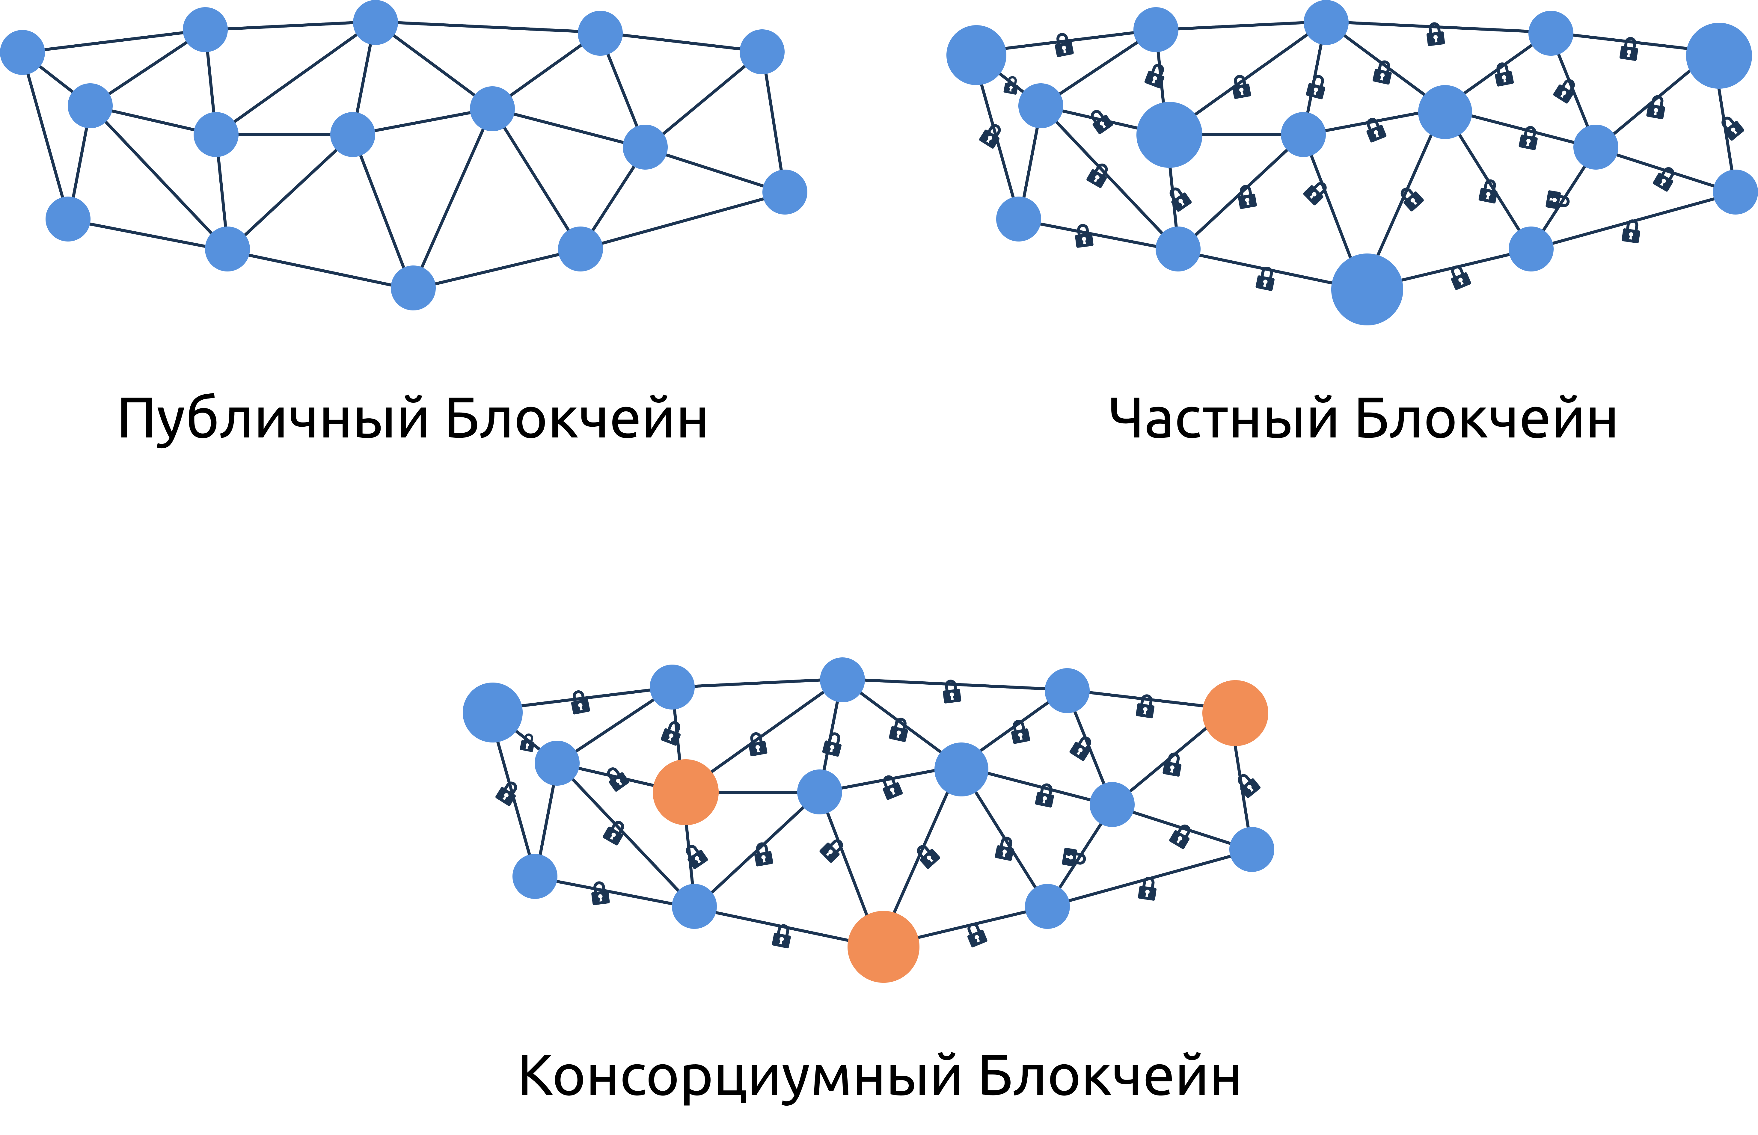
\includegraphics[width=\textwidth]{images/1.types_of_blockchains.png}
	\parskip=6pt
	\caption{Ключевые типы блокчейнов}
	\label{fig:types_of_blockchains}
\end{figure}

Публичные блокчейны представляют собой открытые децентрализованные системы, в которых каждый участник имеет доступ к процессу верификации и валидации транзакций. Эти системы характеризуются высоким уровнем прозрачности и демократичности, позволяя каждому участнику сети взаимодействовать, консенсусно~\cite{bib:consensus} подтверждать и проверять записи в блокчейне. Примером публичного блокчейна является сеть Ethereum~\cite{bib:ethereum}.

Частные блокчейны, напротив, являются закрытыми системами с тщательно регулируемым уровнем доступа и правами участников. В таких системах централизованный администратор или определенная группа лиц контролирует процесс верификации и валидации транзакций, что обеспечивает конфиденциальность и защиту данных. Частные блокчейны часто используются в корпоративных и конфиденциальных системах.

Консорциумные блокчейны представляют собой гибридный вариант, сочетающий элементы публичных и частных блокчейнов. Управление такой сетью осуществляется несколькими определенными организациями, что обеспечивает сбалансированный уровень доверия, децентрализации и контроля в системе. Этот тип блокчейна применяется в межорганизационных проектах.

Применительно к NFT-дипломам, стоит выбирать консорциумные или публичные блокчейны, поскольку в частном блокчейне отсутствует требуемый уровень децентрализации и верификации со стороны независимых участников, что дает возможность организаторам учебного процесса фальсифицировать данные без возможности проведения независимой проверки. Подробное сравнение приведено в таблице~\ref{tab:blockchain_comparison}.

\begin{table}[H]
    \caption{Сравнительная таблица типов блокчейнов для NFT-дипломов}
    \centering

    \tolerance=0
    \emergencystretch=10pt
    \hyphenpenalty=0
    \exhyphenpenalty=0
    \begin{tabular}{x{6cm}x{3cm}x{3cm}x{3cm}}
        \toprule
        \textbf{Характеристика} & \textbf{Публичный блокчейн} & \textbf{Частный блокчейн} & \textbf{Консорциумный блокчейн} \\ \midrule
        Уровень децентрализации & Высокий & Низкий & Средний \\
        Прозрачность & Высокая & Низкая & Средняя \\
        Доступность & Открытый доступ для всех & Доступ ограничен администраторами & Доступ ограничен несколькими организациями \\
        Безопасность & Высокая, за счет децентрализации & Высокая, за счет контроля доступа & Высокая, за счет совместного управления \\
        Конфиденциальность & Низкая & Высокая & Средняя \\
        Скорость транзакций & Ниже, зависит от нагрузки сети & Высокая, благодаря контролируемому доступу & Средняя, баланс между скоростью и децентрализацией \\
        Масштабируемость & Ограниченная & Высокая & Средняя \\
        Примеры использования & Ethereum, Siberium & Hyperledger Fabric & R3 Corda, Мастерчейн \\
        Подходит для NFT-дипломов & Да, благодаря прозрачности и независимой верификации & Нет, из-за отсутствия полноценной децентрализации & Да, благодаря сбалансированному уровню доверия и контроля \\
        \bottomrule
    \end{tabular}
    \label{tab:blockchain_comparison}
\end{table}

\subsubsection{Преимущества и недостатки блокчейн-технологий}

Одним из ключевых преимуществ блокчейн-технологий является надежность и защищенность систем. Использование криптографического шифрования обеспечивает защиту данных, сохраняя подлинность и целостность образовательных документов.

Благодаря распределенной сети блоков минимизируются риски потери данных из-за сбоев в работе или целенаправленных атак на централизованные серверы. В таблице~\ref{tab:blockchain_in_education} приведен подробный анализ, который сопоставляет преимущества и недостатки применения блокчейна в образовании.

\begin{table}[H]
    \caption{Преимущества и недостатки применения блокчейн-технологий в образовании}
    \centering

    \tolerance=0
    \emergencystretch=10pt
    \hyphenpenalty=0
    \exhyphenpenalty=0
    \begin{tabular}{x{3cm}x{6cm}x{6cm}}
        \toprule
        \textbf{Параметр} & \textbf{Преимущество} & \textbf{Недостаток} \\ \midrule
        Прозрачность и Верификация & Блокчейн обеспечивает прозрачность и возможность верификации академических данных, что уменьшает вероятность мошенничества с документами и подтверждает подлинность дипломов. & Избыток прозрачности может вызвать проблемы с конфиденциальностью данных, если не реализованы соответствующие механизмы защиты. \\
        Устойчивость к Изменениям & Благодаря децентрализации блокчейн, зарегистрированные данные не могут быть изменены или удалены, что обеспечивает высокую степень защиты от фальсификаций. & В то же время, это может создать проблемы, если потребуется корректировка данных по каким-то причинам. \\
        Глобальное Признание и Переносимость & Блокчейн-сертификаты могут быть легко доступны и признаны на международном уровне, облегчая мобильность студентов и узнаваемость вуза. & Отсутствие глобальных стандартов и регулирующих рамок может вызвать проблемы с признанием и использованием блокчейн-дипломов в разных странах и учебных заведениях. \\
        Непрерывность доступа к данным & Блокчейн обеспечивает постоянный доступ к данным, что минимизирует риски их утраты из-за сбоев в работе серверов или атак. & Возможны проблемы с масштабируемостью сети при значительном увеличении объема данных и количества пользователей. \\
        Интеграция с существующими системами & Блокчейн может быть интегрирован с существующими системами управления данными, улучшая их безопасность и эффективность. & Трудности интеграции могут возникнуть из-за несовместимости технологий и необходимости модернизации существующей инфраструктуры. \\ 
        \bottomrule
    \end{tabular}
    \label{tab:blockchain_in_education}
\end{table}

Основываясь на собранных данных, можно заключить, что внедрение технологии блокчейн для NFT-дипломов в образовательной сфере представляет собой значительный шаг в сторону модернизации и улучшения управления академическими данными. Преимущества, такие как прозрачность, верификация, устойчивость к фальсификации, децентрализация, экономия ресурсов и глобальное признание, могут значительно повысить эффективность и надежность процессов выдачи и верификации дипломов. Это, в свою очередь, может улучшить репутацию учебных заведений на международном уровне.

Хотя некоторые недостатки, такие как отсутствие глобальных стандартов, требуют внимания, преимущества, которые блокчейн может принести в образовательную сферу, делают его привлекательным вариантом для внедрения NFT-дипломов в высших учебных заведениях.

\subsubsection{Смарт-контракты}

Умные контракты --- это самоисполняющиеся программы, предназначенные для автоматического выполнения и верификации сделок или иных действий при наступлении заранее определенных условий. В контексте образовательного процесса умные контракты могут существенно способствовать автоматизации, прозрачности и надежности процедур верификации и учета академических достижений.~\cite{bib:smart_contract}

Применение умных контрактов позволяет минимизировать влияние человеческого фактора и снижает риск возникновения ошибок или манипуляций с данными со стороны недобросовестных участников процесса. Эти контракты могут автоматизировать процессы выдачи и проверки подлинности дипломов, сертификатов и других образовательных документов.

К сожалению, использование умных контрактов сопряжено с рядом сложностей и ограничений. Во-первых, для разработки, внедрения и поддержки умных контрактов требуется глубокая техническая экспертиза. Во-вторых, умные контракты функционируют строго в соответствии с заложенной в них логикой, что ограничивает их гибкость и адаптивность к изменяющимся обстоятельствам или нестандартным ситуациям без дополнительных модификаций.

\subsection{Инструменты токенизации и виды токенов}

Токенизация~\cite{bib:tokenizer} представляет собой процесс преобразования прав на физический или цифровой актив в цифровой токен на блокчейне. В контексте образования токенизация может использоваться для управления академическими достижениями, дипломами и сертификатами. Существует несколько видов токенов, каждый из которых обладает уникальными характеристиками и применениями.

\subsubsection{Невзаимозаменяемые токены (NFT)}

NFT (Non-Fungible Tokens)~\cite{bib:what_is_nft} --- это уникальные цифровые токены, которые представляют собой собственность на определенный объект или актив. В образовательной сфере NFT могут быть использованы для подтверждения подлинности и уникальности дипломов, сертификатов и других академических достижений.

\textbf{Преимущества и недостатки:}
\begin{itemize}
    \item Каждый NFT представляет собой уникальный актив, что исключает возможность подделки.
    \item Все транзакции с NFT записываются в блокчейн, обеспечивая прозрачность и легкость верификации.
    \item NFT могут быть легко переданы от одного владельца к другому, упрощая процесс обмена и проверки документов.
    \item Создание и управление NFT требует значительных вычислительных ресурсов и может быть дорогостоящим.
    \item Не все платформы и блокчейны поддерживают NFT, что может создавать барьеры для их широкого использования.
\end{itemize}

\subsubsection{Soulbound токены (SBT)}

SBT (Soulbound Tokens)~\cite{bib:what_is_sbt} --- это непередаваемые токены, привязанные к личности владельца. Они предназначены для хранения и подтверждения личных данных и достижений, которые не могут быть переданы или проданы.

\textbf{Преимущества и недостатки:}
\begin{itemize}
    \item SBT гарантирует, что токены не могут быть переданы или проданы, что делает их идеальными для подтверждения личных академических достижений.
    \item Поскольку SBT не могут быть переданы, они снижают риск мошенничества и подделки документов.
    \item Невозможность передачи токенов ограничивает их применение в ситуациях, требующих обмена данными между различными субъектами.
    \item Поскольку SBT привязаны к личности, потеря доступа к ним может привести к утрате важных данных.
\end{itemize}

\subsubsection{Утилитарные токены (Utility Tokens)}

Утилитарные токены~\cite{bib:what_is_utt} --- это цифровые токены, которые предоставляют доступ к определенным услугам или функциональности внутри определенной экосистемы. В образовательной сфере utility токены могут использоваться для доступа к образовательным ресурсам, оплате курсов или участию в обучающих программах.

\textbf{Преимущества и недостатки:}
\begin{itemize}
    \item Утилитарные токены могут использоваться для доступа к различным образовательным ресурсам и услугам.
    \item Эти токены могут быть использованы в различных контекстах и для различных целей, что делает их универсальными.
    \item Утилити токены имеют ограниченное применение за пределами своей экосистемы.
    \item Стоимость токенов может быть подвержена волатильности, что создает финансовые риски для пользователей.
\end{itemize}

\subsection{Система децентрализованного хранения данных (IPFS)}

Межпланетная файловая система (IPFS)~\cite{bib:ipfs} это децентрализованная технология хранения данных. IPFS функционирует как распределенная файловая система, позволяющая хранить и обмениваться файлами в одноранговой сети. Эта заменяет централизованные серверова, распределяя данные по множеству узлов сети, что повышает устойчивость к сбоям и атакам и снижает риск потери данных. Принцип работы HTTP и IPFS приведен на рисунке~\ref{fig:http_vs_ipfs}.

\begin{figure}[H]   
	\centering
	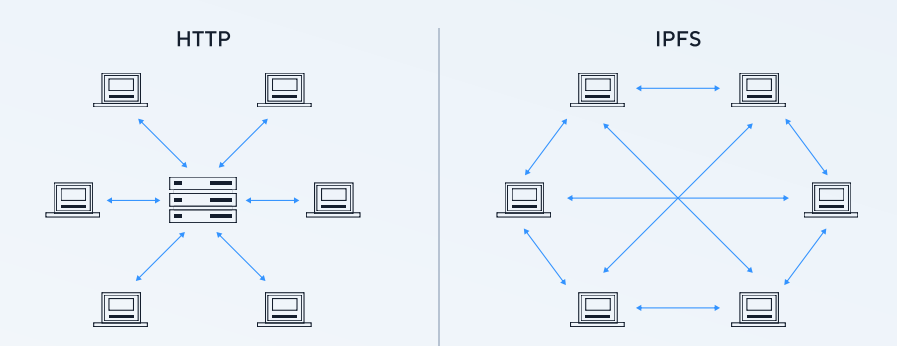
\includegraphics[width=\textwidth]{images/1.http_vs_ipfs.png}
	\parskip=6pt
	\caption{Сравнение HTTP с IPFS обменом данных}
	\label{fig:http_vs_ipfs}
\end{figure}

Одной из ключевых функций IPFS является контент-адресация~\cite{bib:ipfs_2}, где данные идентифицируются не по их расположению, а по содержимому, используя уникальные хэш-коды. Это обеспечивает неизменность данных и облегчает их верификацию, что особенно важно для хранения академических документов. Кроме того, IPFS использует дедупликацию~\cite{bib:dedup}, храня одинаковые данные только один раз, что экономит пространство и ресурсы, снижая дублирование данных. Масштабируемость системы позволяет легко расширяться по мере добавления новых узлов и данных, что обеспечивает возможность обработки больших объемов информации без потери производительности.

В образовательной сфере IPFS может быть использована для хранения студенческих записей, дипломов, сертификатов и других важных академических документов. Такое решение обеспечивает надежность и долговечность хранения данных, минимизируя риск их утраты или повреждения. Преподаватели и студенты могут легко обмениваться учебными материалами и результатами исследований, что упрощает доступ к ресурсам и улучшает сотрудничество между участниками образовательного процесса.

\subsection{Анализ существующих систем}

Одной из первых организаций, внедривших блокчейн в образование, стал Массачусетский технологический институт (MIT). Выпускники MIT могут выбрать получение цифровой версии диплома бесплатно. Этот диплом отправляется в виде вложения к электронному письму, закодированного и поддающегося проверке с помощью технологии Blockcerts. Разработанная в сотрудничестве с компанией Learning Machine, эта технология использует блокчейн для защиты и верификации дипломов.~\cite{bib:mit_diplomas}

Ещё одним примером внедрения блокчейн-технологий является проект социальной сети ВКонтакте (VK), направленный на использование открытого блокчейна Polygon~\cite{bib:polygon} для выдачи NFT-дипломов. ВКонтакте разработала систему, позволяющую университетам выдавать цифровые дипломы и сертификаты в форме NFT не покидая социальной сети.~\cite{bib:vk_nft_diploma}

Московский физико-технический институт (МФТИ) также активно применяет блокчейн-технологии в образовательном процессе. МФТИ разработал и внедрил систему на основе Bitcoin и один из первых в России выдал студентам NFT.~\cite{bib:mipt_nft_diploma}

В таблице~\ref{tab:nft_diplomas_comparison} приведено общее сравнение предлагаемых решений.

\begin{table}[H]
    \caption{Cравнительная таблица систем NFT-дипломов}
    \centering

    \tolerance=0
    \emergencystretch=10pt
    \hyphenpenalty=0
    \exhyphenpenalty=0
    \begin{tabular}{x{4cm}x{3.2cm}x{3.2cm}x{3.2cm}}
        \toprule
        \textbf{Параметр} & \textbf{MIT} & \textbf{ВКонтакте (VK)} & \textbf{МФТИ} \\ \midrule
        Стоимость выпуска и владения & Высокие начальные затраты, низкие эксплуатационные & Средние затраты на выпуск, низкие эксплуатационные & Высокие начальные и эксплуатационные затраты \\
        Применяемый блокчейн & Публичный блокчейн, Blockcerts & Публичный блокчейн, Polygon & Публичный блокчейн, Bitcoin \\
        Вид токена & SBT & SBT & NFT \\
        Прозрачность и контроль & Возможность публичного аудита & Публичный аудит & Публичный аудит, управление доступом \\
        Удобство использования & Интеграция в личный кабинет & Интеграция в профиль & Публичная сеть блокчейн \\
        Конфиденциальность & Высокий & Нет защиты персональных данных & Высокий \\
        Интероперабельность & Низкая & Средняя & Низкая \\
        Пользовательский опыт & Удобный интерфейс для администраторов и студентов & Интуитивный интерфейс, интеграция с соцсетями & Интеграция с существующими LMS \\
        Модульность & Возможность добавления новых модулей и функций & Ограниченные возможности для расширения & Высокая возможность для добавления новых функций \\ \bottomrule
    \end{tabular}
    \label{tab:nft_diplomas_comparison}
\end{table}

